% =====================================================================
% Capítulo: Propuesta (AST-CC)
% =====================================================================

\chapter{AST-CC y el refinamiento jerárquico de ST-CC guiado por pruebas de hipótesis}\label{chap:propuesta}

El capítulo anterior dejó un problema abierto. ST-CC resume cada bloque de su
tablero con un solo valor, de modo que la interacción entre regiones y horarios
que queda dentro de los bloques, el término (iii) de la
Proposición~\ref{prop:descomposicion}, permanece sin modelar, y un patrón local,
como unas pocas regiones que se activan solo en ciertos horarios, queda diluido
dentro de un bloque que parece uniforme. Resolverlo exige dos cosas, que son una
forma de subdividir un bloque sin alterar el resto de la matriz y un criterio
estadístico para decidir si esa subdivisión refleja un patrón real o ruido, y para
saber cuándo detenerse.

Este capítulo presenta el método propuesto, al que se denomina \emph{Adaptive
Spatio-Temporal Co-Clustering} (AST-CC). El método conserva la partición en
tablero que produce ST-CC y la toma como punto de partida de un árbol de
refinamientos locales, en el que cada bloque se examina por separado y, si contiene
interacción residual entre regiones y horarios que sea estadísticamente
detectable y de tamaño relevante, se subdivide; en caso contrario, se conserva
como hoja.

El capítulo sigue el mismo orden lógico que el anterior, de lo general a lo
específico. Primero se da una visión general del método. Luego se formaliza el
refinamiento como un árbol de bloques y se demuestra que la función objetivo se
descompone de forma exacta por hojas, lo que convierte la ganancia de cada corte
en un estadístico de razón de verosimilitud. Sobre esa base se definen los
estadísticos de heterogeneidad, la regla de decisión, la calibración de las
pruebas, el control de comparaciones múltiples y los criterios de parada. El
capítulo termina con el algoritmo completo, su costo computacional, la forma de
presentar los resultados y las limitaciones del diseño.

\section{Visión general}\label{sec:prop-vision}

La idea central de AST-CC puede resumirse en que se debe refinar mientras haya
heterogeneidad local estadísticamente detectable y de tamaño relevante, y
detenerse cuando todas las hojas sean indistinguibles de su modelo nulo local.
Esta idea es la traducción al objeto bidimensional del principio de SigTree
\cite{Hu2025}, que detiene el crecimiento de su árbol cuando ninguna división
candidata es significativa. Para llevarla a la práctica, el método se organiza en
cuatro etapas, que se ilustran en la Figura~\ref{fig:prop-teselacion} y se
describen a continuación.

\begin{enumerate}
  \item \textbf{Construcción de la matriz.} Los viajes se agregan en una
  matriz $O \in \mathbb{N}^{m\times n}$ de conteos totales región $\times$
  intervalo de tiempo, y se conservan además las $D$ matrices diarias cuya
  suma es $O$, que se usan para calibrar las pruebas. Se usan conteos y no
  promedios diarios, por la razón expuesta en la Sección~\ref{sec:escala}, ya que
  solo sobre conteos la I-divergencia coincide con la devianza de Poisson.
  \item \textbf{Partición base.} Se ejecuta BBAC$_I$ con $K_R$ grupos de
  filas y $K_T$ grupos de columnas y la base C5 adoptada en la
  Sección~\ref{sec:stcc-base}, desde varias inicializaciones y con una
  búsqueda local que mueve filas y columnas de una en una
  (Sección~\ref{sec:bbac-algoritmo}). El resultado es un tablero del mismo tipo
  que el de ST-CC, aunque no necesariamente el mismo, porque la implementación
  de ST-CC corresponde a la base C2.
  \item \textbf{Refinamiento.} Cada uno de los $K_R K_T$ bloques se somete a
  un procedimiento recursivo que decide, mediante pruebas de hipótesis, si se
  divide por filas, por columnas, de forma conjunta, o si se convierte en hoja.
  \item \textbf{Resumen.} Las hojas del árbol se describen con su tamaño de
  efecto y su nivel de actividad respecto de los volúmenes globales de sus
  regiones e intervalos, y se representan de forma que se conserve la lectura
  espacial y temporal que ofrece ST-CC.
\end{enumerate}

\begin{figure}[t]
\centering
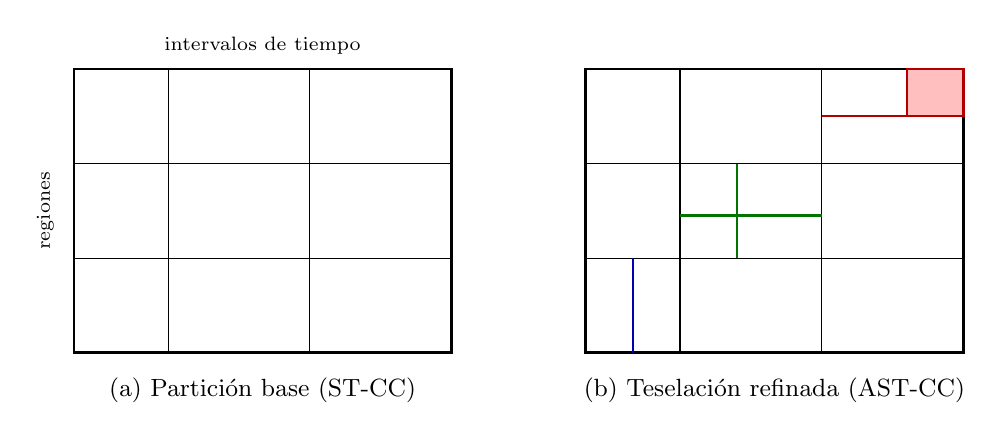
\begin{tikzpicture}[x=0.6cm,y=0.6cm]
  % ---- Panel izquierdo: tablero de ST-CC ----
  \begin{scope}
    \draw[thick] (0,0) rectangle (8,6);
    \foreach \x in {2,5} \draw (\x,0) -- (\x,6);
    \foreach \y in {2,4} \draw (0,\y) -- (8,\y);
    \node at (4,-0.8) {\small (a) Partición base (ST-CC)};
    \node[rotate=90] at (-0.6,3) {\scriptsize regiones};
    \node at (4,6.5) {\scriptsize intervalos de tiempo};
  \end{scope}
  % ---- Panel derecho: teselación refinada ----
  \begin{scope}[xshift=6.5cm]
    \draw[thick] (0,0) rectangle (8,6);
    \foreach \x in {2,5} \draw (\x,0) -- (\x,6);
    \foreach \y in {2,4} \draw (0,\y) -- (8,\y);
    % bloque (fila 1, col 3): corte de filas y luego corte de columnas
    \draw[red!70!black, thick] (5,5) -- (8,5);
    \draw[red!70!black, thick] (6.8,5) -- (6.8,6);
    \fill[red!25] (6.8,5) rectangle (8,6);
    \draw[red!70!black, thick] (6.8,5) rectangle (8,6);
    % bloque (fila 3, col 1): corte de columnas
    \draw[blue!70!black, thick] (1,0) -- (1,2);
    % bloque (fila 2, col 2): corte conjunto 2x2
    \draw[green!45!black, thick] (3.2,2) -- (3.2,4);
    \draw[green!45!black, thick] (2,2.9) -- (5,2.9);
    \node at (4,-0.8) {\small (b) Teselación refinada (AST-CC)};
  \end{scope}
\end{tikzpicture}
\caption{Comparación entre la partición en tablero de ST-CC y la teselación que
produce AST-CC. En (b), un bloque se refinó con un corte de filas seguido de un
corte de columnas (rojo; la hoja sombreada representa un patrón local), otro con
un corte de columnas (azul) y otro con un corte conjunto $2\times 2$ (verde).
Los cortes solo afectan al bloque en que se producen, por lo que el resultado
deja de ser una rejilla global.}
\label{fig:prop-teselacion}
\end{figure}

La diferencia con aumentar $K_R$ y $K_T$ es visible en la figura. En una
rejilla global, cada nuevo corte atraviesa toda la matriz y fragmenta también las
zonas que no presentan ningún patrón de interés, mientras que en AST-CC cada corte
afecta solo al bloque donde se detectó la heterogeneidad. Por esta razón, el
número de parámetros que añade el refinamiento crece con la cantidad de estructura
local encontrada y no con la resolución global de la partición, lo que permite
capturar un patrón fino en una zona de la matriz sin pagar el costo de dividir
las demás.

\section{Formulación del refinamiento}\label{sec:prop-formulacion}

\subsection{Notación}

Se mantiene la notación del Capítulo~\ref{chap:marco}. Un bloque es un
producto $B = I \times J$ con $I \subseteq \{1,\dots,m\}$ y
$J \subseteq \{1,\dots,n\}$. Para un bloque se definen sus totales internos
\[
  O^{B}_{i\cdot} = \sum_{j\in J} O_{ij}\ (i\in I), \qquad
  O^{B}_{\cdot j} = \sum_{i\in I} O_{ij}\ (j\in J), \qquad
  N_B = \sum_{(i,j)\in B} O_{ij},
\]
y los conteos esperados bajo independencia entre filas y columnas dentro del
bloque,
\begin{equation}\label{eq:prop-EB}
  E^{B}_{ij} = \frac{O^{B}_{i\cdot}\, O^{B}_{\cdot j}}{N_B},
  \qquad (i,j)\in B .
\end{equation}
El estadístico de razón de verosimilitud de la prueba de independencia en el
bloque y la información mutua empírica asociada son, como en
\eqref{eq:c6-g2} y \eqref{eq:g2-im},
\begin{equation}\label{eq:prop-G2}
  G^2_B = 2\sum_{(i,j)\in B} O_{ij}\log\frac{O_{ij}}{E^{B}_{ij}},
  \qquad
  \hat I_B = \frac{G^2_B}{2N_B}.
\end{equation}
La cantidad $\hat I_B$ se mide en nats por observación, no crece con el
tamaño de la muestra y, en una versión corregida por sesgo
(Sección~\ref{sec:prop-parada}), se usará como tamaño de efecto. Conviene no
confundir $G^2_B$, que mide la heterogeneidad total del bloque, con $G^2_{B,s}$,
que se define más adelante y mide la parte de esa heterogeneidad que explica un
corte concreto $s$.

\subsection{Árbol de bloques y teselación guillotina}

El objeto que optimiza AST-CC deja de ser un par de mapeos $(\rho,\tau)$ y pasa
a ser un árbol de bloques anidados. Cada bloque del árbol se subdivide mediante un
corte que solo actúa dentro de él, de modo que el resultado final es una partición
de la matriz en rectángulos con la estructura de teselación guillotina descrita en
el Capítulo~\ref{chap:marco}. Las definiciones siguientes formalizan los cortes
posibles y el árbol que resulta de aplicarlos.

\begin{definicion}[Corte de un bloque]\label{def:corte}
Un corte $s$ de un bloque $B = I\times J$ es una partición de $B$ en
bloques hijos de uno de tres tipos, que se enumeran a continuación.
\begin{enumerate}
  \item Corte de filas, que produce los hijos $\{I_1\times J,\ I_2\times J\}$, con
  $\{I_1,I_2\}$ partición de $I$;
  \item corte de columnas, que produce los hijos $\{I\times J_1,\ I\times J_2\}$, con
  $\{J_1,J_2\}$ partición de $J$;
  \item corte conjunto, que produce los hijos $\{I_a\times J_b\}_{a,b\in\{1,2\}}$, con
  $\{I_1,I_2\}$ y $\{J_1,J_2\}$ particiones de $I$ y de $J$.
\end{enumerate}
Se denota $\mathcal{C}(B,s)$ al conjunto de hijos.
\end{definicion}

\begin{definicion}[Árbol de refinamiento]\label{def:arbol}
Un árbol de refinamiento $\mathcal{T}$ es un árbol con raíz en el que
\begin{enumerate}
  \item los hijos de la raíz son los $K_R K_T$ bloques
  $B_{gh} = I_g\times J_h$ de la partición base $(\rho,\tau)$;
  \item cada nodo interno $B$ tiene como hijos los bloques
  $\mathcal{C}(B,s_B)$ de un corte $s_B$.
\end{enumerate}
El conjunto de hojas se denota $\mathcal{L}(\mathcal{T})$.
\end{definicion}

Por construcción, $\mathcal{L}(\mathcal{T})$ es una partición de
$\{1,\dots,m\}\times\{1,\dots,n\}$ en rectángulos (en el sentido de
subconjuntos de filas por subconjuntos de columnas) con estructura de
guillotina anidada. Cuando el árbol no tiene nodos internos por debajo de la
partición base, $\mathcal{L}(\mathcal{T})$ coincide con el tablero de ST-CC.
Dos filas que pertenecen al mismo grupo base pueden terminar en hojas con
particiones temporales distintas; esta es precisamente la flexibilidad que se
busca.

\subsection{Modelo local y aproximación}

A cada árbol se le asocia una aproximación de la matriz. La elección coherente
con el Capítulo~\ref{chap:marco} es modelar cada hoja con el modelo de
independencia de su propio bloque. Esta elección tiene la ventaja de que cada hoja
se ajusta con su propio efecto de fila y de columna, de modo que la aproximación
no se ve afectada por las diferencias de volumen entre las regiones o los
horarios que la componen, que es justamente la propiedad que justificó, en la
Proposición~\ref{prop:descomposicion}, el uso del estadístico $G^2$ como medida
de la interacción local.

\begin{definicion}[Aproximación de un árbol]\label{def:aprox-arbol}
Para $(i,j)$, sea $L(i,j)\in\mathcal{L}(\mathcal{T})$ la hoja que la contiene.
La aproximación asociada a $\mathcal{T}$ es
\[
  \hat O^{\mathcal{T}}_{ij} = E^{L(i,j)}_{ij}
  = \frac{O^{L}_{i\cdot}\, O^{L}_{\cdot j}}{N_L}\,,\qquad L = L(i,j).
\]
\end{definicion}

Cuando las hojas son los bloques base, $\hat O^{\mathcal{T}}$ es la
aproximación de la base C6 \cite{Banerjee2007} para la partición $(\rho,\tau)$.
En general, $\hat O^{\mathcal{T}}$ es el estimador de máxima verosimilitud de un
modelo log-lineal de Poisson en el que cada hoja tiene sus propios efectos de
fila y de columna, con $\sum_{L}(|I_L|+|J_L|-1)$ parámetros libres.

\subsection{Descomposición por hojas y ganancia de un corte}\label{sec:prop-descomp}

El siguiente resultado es la pieza que hace viable el esquema recursivo, pues la
divergencia del árbol se reparte exactamente entre sus hojas, y la reducción que
produce un corte es un estadístico de razón de verosimilitud que puede evaluarse
localmente. Dado que el árbol se construye de forma voraz, de arriba abajo, esta
propiedad es la que garantiza que decidir cada corte con la información de su
propio bloque es coherente con la función objetivo global.

\begin{proposicion}[Descomposición por hojas y ganancia de un corte]\label{prop:ganancia}
Sea $\mathcal{T}$ un árbol de refinamiento y supóngase que $E^{B}_{ij}>0$
siempre que $O_{ij}>0$.
\begin{enumerate}
  \item[(a)] La divergencia del árbol se descompone por hojas,
  \begin{equation}\label{eq:prop-desc-hojas}
    D_I\bigl(O \,\|\, \hat O^{\mathcal{T}}\bigr)
    = \frac12 \sum_{L\in\mathcal{L}(\mathcal{T})} G^2_L .
  \end{equation}
  \item[(b)] Si un bloque $B$ se divide mediante un corte $s$, entonces
  \begin{equation}\label{eq:prop-cadena}
    G^2_B = G^2_{B,s} + \sum_{C\in\mathcal{C}(B,s)} G^2_C ,
  \end{equation}
  donde $G^2_{B,s}\ge 0$ es el estadístico de razón de verosimilitud que
  compara la independencia en $B$ con el modelo en que cada hijo tiene sus
  propios efectos de fila y columna. Para un corte de filas
  $\{I_1, I_2\}$, con $O_{rj} = \sum_{i\in I_r} O_{ij}$ y
  $N_r = \sum_{j\in J} O_{rj}$,
  \begin{equation}\label{eq:prop-G2-colapsada}
    G^2_{B,s} = 2\sum_{r=1}^{2}\sum_{j\in J} O_{rj}
      \log\frac{O_{rj}\,N_B}{N_r\,O^{B}_{\cdot j}},
  \end{equation}
  que es el estadístico $G^2$ de independencia de la tabla colapsada
  $2\times|J|$. El caso de columnas es simétrico. Los grados de libertad
  asintóticos de $G^2_{B,s}$ son $|J|-1$ para un corte de filas, $|I|-1$
  para uno de columnas y $|I|+|J|-3$ para uno conjunto.
  \item[(c)] En consecuencia, sustituir la hoja $B$ por sus hijos reduce la
  divergencia del árbol exactamente en $\tfrac12\, G^2_{B,s}$.
\end{enumerate}
\end{proposicion}

\begin{proof}
(a) Dentro de cada hoja, la aproximación reproduce el total $N_L$, de modo que
$\sum_{(i,j)\in L}(O_{ij}-E^{L}_{ij}) = 0$ y los términos lineales de la
I-divergencia se cancelan. Queda
$\sum_{(i,j)\in L} d_I(O_{ij},E^L_{ij}) = \sum_{(i,j)\in L} O_{ij}\log(O_{ij}/E^L_{ij}) = \tfrac12 G^2_L$,
y basta sumar sobre las hojas.

(b) Restringido a $B$, el modelo de independencia,
$\log\mu_{ij} = \alpha_i + \beta_j$, está anidado en el modelo del corte. Para
un corte de filas, este último es $\log\mu_{ij} = \alpha_i + \beta_{r(i),j}$,
donde $r(i)$ indica el hijo de la fila $i$; para uno conjunto, es
$\log\mu_{ij} = \alpha_{i,b(j)} + \beta_{a(i),j}$, que es la base C6 restringida
al bloque. En los tres casos, la estimación de máxima verosimilitud del modelo
del corte coincide, sobre cada hijo $C$, con su aproximación de independencia
$E^{C}$. La identidad pitagórica usada en la demostración de la
Proposición~\ref{prop:descomposicion}, aplicada al par de modelos anidados,
da
\[
  D_I(O|_B \,\|\, E^{B})
  = \sum_{C\in\mathcal{C}(B,s)} D_I(O|_C \,\|\, E^{C})
  + D_I(\hat E^{B,s} \,\|\, E^{B}),
\]
donde $\hat E^{B,s}$ es la aproximación del modelo del corte. Multiplicando por
dos y usando (a) se obtiene \eqref{eq:prop-cadena} con
$G^2_{B,s} = 2D_I(\hat E^{B,s}\|E^B)$. Para un corte de filas, los totales de
fila de cada hijo coinciden con los de $B$, y
$\log(E^{C_r}_{ij}/E^{B}_{ij}) = \log\bigl(O_{rj}N_B/(N_r O^B_{\cdot j})\bigr)$
no depende de $i$; al sumar sobre $i\in I_r$ se obtiene
\eqref{eq:prop-G2-colapsada}. Los grados de libertad son la diferencia en el
número de parámetros libres, que son $|I|+|J|-1$ para la independencia en $B$ frente a
$\sum_C(|I_C|+|J_C|-1)$ para el modelo del corte.

(c) Se sigue de (a) y (b), porque los términos de las demás hojas no cambian.
\end{proof}

Un ejemplo numérico muestra cómo funciona el reparto. Sea un bloque de cuatro
regiones y dos horarios con conteos $(30,10)$, $(28,12)$, $(10,30)$ y $(12,28)$
por fila, de modo que $N_B = 160$ y todos los conteos esperados valen 20. Su
estadístico es $G^2_B\approx 34.10$ con tres grados de libertad, y su
información mutua, $\hat I_B\approx 0.107$ nats por observación. Un corte de
filas en $\{1,2\}$ y $\{3,4\}$ colapsa el bloque en la tabla $(58,22)$ y
$(22,58)$, cuyo estadístico es $G^2_{B,s}\approx 33.59$ con un grado de libertad,
mientras que cada hijo conserva solo $G^2_C\approx 0.25$. La suma
$33.59 + 0.25 + 0.25$ reproduce $G^2_B$ salvo redondeo, y el corte explica cerca
del 98.5\,\% de la heterogeneidad del bloque a cambio de un único parámetro
adicional, ya que la independencia en $B$ usa $4+2-1=5$ parámetros y los dos
hijos usan $3+3=6$. Un corte de columnas separaría las dos columnas y explicaría
todo el estadístico, pero con tres grados de libertad, lo que ilustra por qué
la comparación entre tipos de corte se hace con p-valores calibrados y no con
valores crudos de $G^2_{B,s}$.

La proposición admite una lectura informacional directa. Dividiendo
\eqref{eq:prop-cadena} entre $2N_B$, para un corte de filas se obtiene
\begin{equation}\label{eq:prop-regla-cadena}
  \hat I_B(R;T) = \hat I_B(\hat R_s;T)
  + \sum_{r=1}^{2}\frac{N_r}{N_B}\,\hat I_{C_r}(R;T),
\end{equation}
que es la regla de la cadena de la información mutua, con $\hat R_s$ el grupo de
filas inducido por el corte. La asociación que hay dentro de un bloque se
reparte, sin pérdida ni duplicación, entre la parte que el corte explica y la
que queda dentro de los hijos.

\begin{corolario}[Relación con la función objetivo de ST-CC]\label{cor:stcc}
Sea $\mathcal{S}(\mathcal{T})$ el conjunto de nodos internos de $\mathcal{T}$
por debajo de la partición base, con sus cortes $s_B$. Entonces
\begin{equation}\label{eq:prop-desc-total}
  D_I\bigl(O\,\|\,\hat O^{C2}\bigr)
  = \underbrace{\text{(i)} + \text{(ii)}}_{\text{Prop.~\ref{prop:descomposicion}}}
  + \underbrace{\frac12\sum_{B\in\mathcal{S}(\mathcal{T})} G^2_{B,s_B}}_{\text{estructura local explicada}}
  + \underbrace{\frac12\sum_{L\in\mathcal{L}(\mathcal{T})} G^2_L}_{\text{interacción residual}} .
\end{equation}
\end{corolario}

\begin{proof}
El término (iii) de la Proposición~\ref{prop:descomposicion} es
$\tfrac12\sum_{g,h}G^2_{gh}$, es decir, la expresión
\eqref{eq:prop-desc-hojas} para el árbol que solo contiene la partición base.
Aplicando \eqref{eq:prop-cadena} a cada nodo interno, por inducción sobre la
profundidad, ese término se reparte en las dos sumas indicadas.
\end{proof}

El reparto del término (iii) depende solo de la partición en tablero y no del
algoritmo que la encontró, por lo que el corolario es válido para cualquier
tablero, sea que se obtenga con la base C2 o con la base C5 adoptada en esta
tesis. La base solo cambia qué tablero se encuentra y, con él, el valor de cada
término. El corolario sitúa con precisión lo que hace el método. ST-CC deja sin modelar
el término (iii), la interacción espacio-temporal que queda dentro de los
bloques. AST-CC descompone ese término de forma voraz, de modo que cada corte aceptado
traslada una cantidad $\tfrac12 G^2_{B,s}$ desde la interacción residual hacia
la estructura local explicada, y el proceso se detiene cuando lo que queda en
cada hoja no se distingue del ruido. El criterio de refinamiento y la función
objetivo de ST-CC son, por lo tanto, la misma cantidad evaluada a distintos
niveles de granularidad, y no un criterio importado de otro marco.

\subsection{Planteamiento del problema}\label{sec:prop-problema}

Con los elementos anteriores, el problema se formula en su versión restringida
como
\begin{equation}\label{eq:prop-restringido}
  \begin{aligned}
    \mathcal{T}^\ast = \arg\min_{\mathcal{T}}\ \ & D_I\bigl(O\,\|\,\hat O^{\mathcal{T}}\bigr)\\
    \text{sujeto a}\ \ & \text{ninguna hoja } L\in\mathcal{L}(\mathcal{T})
      \text{ presenta heterogeneidad}\\
      & \text{significativa y relevante.}
  \end{aligned}
\end{equation}
La condición sobre las hojas se concreta en la Sección~\ref{sec:prop-decision}
mediante una prueba de hipótesis a un nivel $\alpha_L$ y un umbral de tamaño
de efecto $\delta$. El problema \eqref{eq:prop-restringido} no se resuelve de
forma exacta, ya que AST-CC construye el árbol de forma voraz, de arriba abajo, y
decide cada corte con información local. La Proposición~\ref{prop:ganancia}
garantiza que esas decisiones locales son coherentes con el objetivo global,
pero no que el árbol resultante sea el óptimo.

Como criterio complementario, no frecuentista, se considera también la versión
penalizada
\begin{equation}\label{eq:prop-bic}
  J_\lambda(\mathcal{T}) = D_I\bigl(O\,\|\,\hat O^{\mathcal{T}}\bigr)
  + \lambda \sum_{L\in\mathcal{L}(\mathcal{T})}\bigl(|I_L|+|J_L|-1\bigr),
  \qquad \lambda = \tfrac12\log N,
\end{equation}
que corresponde al criterio BIC por la equivalencia \eqref{eq:devianza} entre
I-divergencia y devianza. Esta versión no se usa para construir el árbol, sino
para comparar, con una misma escala, árboles de AST-CC con rejillas globales de
distinto tamaño, que es la comparación que exige la
Sección~\ref{sec:prop-limitaciones}.

\section{Estadísticos de heterogeneidad}\label{sec:prop-estadisticos}

\subsection{Elección del modelo nulo}

Refinar un bloque requiere decidir frente a qué modelo nulo se juzga su
heterogeneidad, ya que la respuesta depende de qué se considere un comportamiento
esperado dentro del bloque. Esta decisión es importante porque un nulo
demasiado simple rechazaría casi cualquier bloque y el refinamiento no se
detendría, mientras que uno demasiado flexible no detectaría ningún patrón. En
esta tesis se consideraron dos candidatos naturales, que se describen a
continuación.

\begin{itemize}
  \item \textbf{Nulo de constancia.} Supone que $\mu_{ij}=\theta$ para toda
  $(i,j)\in B$, y es el nulo implícito en la base C2, que resume el bloque por
  su media.
  \item \textbf{Nulo de independencia.} Supone que $\mu_{ij} = a_i\, b_j$ dentro de
  $B$, de modo que los conteos del bloque se explican por el producto de un efecto
  de región y un efecto de horario.
\end{itemize}

La Proposición~\ref{prop:descomposicion} resuelve la elección. Un criterio de
constancia mezcla los tres términos de la descomposición y, en datos de
movilidad con volúmenes muy desiguales entre zonas y horarios, rechazaría la
homogeneidad de casi todos los bloques por el término (i), de modo que el
refinamiento solo se detendría al alcanzar los límites de tamaño. El nulo de
independencia aísla el término (iii), de modo que rechazarlo significa que un subconjunto de
regiones se activa en un subconjunto de horarios del bloque de forma distinta
al resto, que es la definición operativa de patrón local que adopta esta
tesis. AST-CC usa, por tanto, el nulo de independencia en todas sus pruebas.
Como la matriz es la suma de $D$ días, el nulo se refiere a las medias del
conteo agregado, $\mathrm{E}[O_{ij}] = a_i b_j$ para $(i,j)\in B$. Un ejemplo
ilustra la diferencia. En un bloque con filas $(80,20)$ y $(40,10)$ la segunda
región tiene la mitad del volumen de la primera pero el mismo perfil horario, de
modo que no hay ningún patrón local. El nulo de constancia, con esperado $37.5$ en
todas las celdas, daría $G^2\approx 74.8$ con tres grados de libertad y lo
rechazaría con claridad, mientras que el de independencia reproduce exactamente
las cuatro celdas y da $G^2 = 0$.

\subsection{Prueba ómnibus}

La primera pregunta sobre un bloque es si contiene algo que refinar. Se
responde con la prueba de independencia sobre la tabla $O|_B$, con estadístico
$G^2_B$ \eqref{eq:prop-G2}. Si los conteos fueran de Poisson independientes, al
condicionar sobre los totales de fila y columna del bloque la tabla seguiría,
bajo el nulo, una distribución hipergeométrica multivariada que no depende de
los parámetros desconocidos $a_i$ y $b_j$, y el p-valor podría calcularse de
forma exacta por simulación (Sección~\ref{sec:est-permutacion}). Los conteos de
taxis, sin embargo, varían entre días mucho más de lo que admite ese modelo, y
de forma correlacionada entre celdas (Sección~\ref{sec:prop-sobredispersion}).
Por ejemplo, con una varianza igual a tres veces la media, el valor típico de
$G^2_B$ bajo el nulo ronda $3\nu$ y no $\nu$, de modo que en un bloque con
$\nu=12$ sin ningún patrón se esperarían unas 36 unidades, y una prueba $\chi^2$
con 12 grados de libertad daría $p<0.001$. Por eso AST-CC genera la distribución
nula remuestreando los días observados (Sección~\ref{sec:prop-bootstrap}), y no usa
la aproximación $\chi^2$ con $(|I|-1)(|J|-1)$ grados de libertad en ningún caso.

\subsection{Pruebas dirigidas}

Si la prueba ómnibus indica heterogeneidad, la segunda pregunta es qué corte la
captura. Para cada tipo de corte se define un estadístico dirigido, el máximo de
la ganancia \eqref{eq:prop-cadena} sobre un conjunto de candidatos,
\begin{equation}\label{eq:prop-dirigidos}
  T_{\mathrm{tipo}}(B) = \max_{s\in\mathcal{S}_{\mathrm{tipo}}(B)} G^2_{B,s},
  \qquad \mathrm{tipo}\in\{\mathrm{fil},\ \mathrm{col},\ \mathrm{conj}\},
\end{equation}
donde $\mathcal{S}_{\mathrm{fil}}(B)$, $\mathcal{S}_{\mathrm{col}}(B)$ y
$\mathcal{S}_{\mathrm{conj}}(B)$ son los conjuntos de cortes candidatos de filas,
de columnas y conjuntos (Sección~\ref{sec:prop-candidatos}).
Dentro de un mismo tipo, todos los candidatos tienen los mismos grados de
libertad, por lo que maximizar $G^2_{B,s}$ equivale a minimizar su p-valor
asintótico. Este es el análogo directo de la elección de la división de menor
p-valor en SigTree \cite{Hu2025}; la diferencia es que la tabla que se prueba
no enfrenta la división con otros atributos, sino con la otra dimensión del
propio bloque. Entre tipos distintos, los grados de libertad difieren y la
comparación se hace mediante p-valores calibrados.

\begin{observacion}[Las tres pruebas comparten la hipótesis nula]\label{obs:nulo-comun}
El bloque satisface el nulo de independencia si y solo si todas sus filas tienen
el mismo perfil sobre las columnas. En ese caso, ningún corte de filas ni de
columnas tiene efecto poblacional; recíprocamente, si ningún corte de filas
tiene efecto, en particular ninguna fila aislada difiere del resto y el bloque
es independiente. Por lo tanto, la prueba ómnibus y las dirigidas contrastan la
misma hipótesis nula con estadísticos de distinta potencia. La consecuencia de
diseño es importante, ya que el error de tipo~I que interesa controlar, declarar
heterogéneo un bloque que no lo es, queda controlado por la prueba ómnibus; las
pruebas dirigidas, que solo se realizan cuando la ómnibus rechaza, cumplen el
papel de localizar la estructura con evidencia suficiente, no el de
añadir nuevas oportunidades de falso rechazo.
\end{observacion}

Conviene señalar un caso que podría parecer problemático. Un patrón en tablero
dentro del bloque, por ejemplo unas zonas activas en la mañana y otras en la
tarde con totales de fila y de columna idénticos, no deja rastro en las
marginales del bloque. Sin embargo, sí lo captura un corte de filas, porque
\eqref{eq:prop-G2-colapsada} compara los perfiles completos de los dos
grupos de filas sobre las columnas, no sus totales. Con las filas $(30,10)$,
$(10,30)$, $(30,10)$ y $(10,30)$, todos los totales de fila valen 40 y los de
columna 80, pero el corte $\{1,3\}$ frente a $\{2,4\}$ colapsa el bloque en
$(60,20)$ y $(20,60)$, con $G^2_{B,s}\approx 41.9$. Los cortes unidimensionales
son, por ello, suficientes para la mayoría de las estructuras; el corte conjunto
se reserva para el caso en que la evidencia está repartida entre ambas
dimensiones (Sección~\ref{sec:prop-decision}).

\subsection{Generación de cortes candidatos}\label{sec:prop-candidatos}

Un bloque con $|I|$ filas admite $2^{|I|-1}-1$ biparticiones de filas, y uno
con $|J|$ columnas, $2^{|J|-1}-1$ de columnas. AST-CC enumera todos los
candidatos siempre que su número es manejable y recurre a una búsqueda
heurística solo por encima de ese límite. Con cuatro filas hay 7 biparticiones,
con catorce hay 8191 y con quince serían 16383, de modo que cada fila adicional
duplica el costo. Los candidatos se generan de forma
distinta para cada tipo de corte y según el tamaño del bloque, como se detalla a
continuación.

\begin{itemize}
  \item \textbf{Columnas.} Con la resolución temporal de ST-CC ($n=12$), un
  bloque tiene a lo sumo $2^{11}-1 = 2047$ biparticiones de columnas, y cada
  $G^2_{B,s}$ se calcula sobre una tabla colapsada $|I|\times 2$. Se enumeran
  todas.
  \item \textbf{Filas.} Si $|I|\le 14$, se enumeran las a lo sumo $8191$
  biparticiones. En bloques mayores se usa una búsqueda heurística, ya que maximizar
  \eqref{eq:prop-G2-colapsada} sobre los cortes de filas equivale a maximizar
  $\hat I_B(\hat R_s;T)$, y como $\hat I_B(R;T)$ es fijo en el bloque, equivale
  a minimizar
  $\sum_{i\in I} O^B_{i\cdot}\,\mathrm{KL}\bigl(p(\cdot\mid i)\,\|\,p(\cdot\mid r(i))\bigr)$,
  donde $p(\cdot\mid i)$ es el perfil de la fila $i$ sobre $J$. Es el paso de
  filas del co-agrupamiento de teoría de la información \cite{Dhillon2003}
  con dos grupos, es decir, un 2-medias con divergencia de Kullback--Leibler
  ponderada, que agrupa las filas por la forma de su perfil horario y no por su
  volumen, y que se ejecuta con $R_{\mathrm{ini}}$ inicializaciones. El límite
  se fijó por dos razones. La primera es que, en una comprobación preliminar sobre
  tablas de ocho filas en las que el óptimo puede calcularse por enumeración, el
  2-medias con diez inicializaciones no lo alcanzó en alrededor del 8\,\% de los
  casos, por lo que conviene enumerar siempre que se pueda. La segunda es el
  costo, ya que cada réplica nula repite la búsqueda y el número de candidatos se
  duplica con cada fila, de modo que catorce filas es el tamaño hasta el cual la
  enumeración sigue siendo manejable con el número de réplicas de la
  Tabla~\ref{tab:prop-parametros}. Con este límite, todos los bloques base de los
  datos de esta tesis, que tienen a lo sumo quince filas, se resuelven de forma
  casi siempre exacta.
  \item \textbf{Conjunto.} Por la identidad \eqref{eq:prop-cadena},
  $G^2_{B,s} = G^2_B - \sum_{C} G^2_C$, de modo que maximizar la ganancia de
  un corte conjunto equivale a minimizar la suma de los $G^2$ de sus cuatro
  hijos. Fijado el corte de columnas, esa suma depende del corte de filas solo
  a través de los totales de columna de cada grupo de filas, y puede
  minimizarse por enumeración. Si $|J|\le 6$ y $|I|\le 14$, se recorren todos
  los cortes de columnas y, para cada uno, se elige el mejor corte de filas, lo
  que da el óptimo exacto. En bloques mayores se alternan los dos pasos, que es
  el algoritmo de la Sección~\ref{sec:bbac-algoritmo} con base C6 y $k=l=2$
  restringido al bloque, desde los mejores cortes de filas y de columnas. El paso
  de filas enumera todos los cortes, de modo que solo se aplica cuando $|I|\le 14$;
  con más filas se conserva el corte de filas inicial del 2-medias y solo se
  actualiza el de columnas.
\end{itemize}

Que una búsqueda sea heurística no compromete la validez de la prueba, siempre
que el mismo procedimiento se repita en cada réplica nula
(Sección~\ref{sec:prop-minP}), pues el p-valor resultante es válido para el
estadístico que efectivamente se calcula, aunque este no sea el máximo exacto.
Lo que se pierde es potencia, y por eso se prefiere la enumeración siempre que
es posible.

\section{Regla de decisión}\label{sec:prop-decision}

La regla combina la prueba ómnibus, las pruebas dirigidas y el umbral de tamaño
de efecto en un procedimiento híbrido, que se resume en la
Figura~\ref{fig:prop-decision}. Sean $\alpha_B$ el nivel asignado al bloque
(Sección~\ref{sec:prop-multiplicidad}), $p_{\mathrm{omn}}$ el p-valor de la
prueba ómnibus y $p_{\mathrm{fil}}$, $p_{\mathrm{col}}$, $p_{\mathrm{conj}}$ los
p-valores calibrados de los estadísticos \eqref{eq:prop-dirigidos}.

\begin{enumerate}
  \item \textbf{Puerta ómnibus.} Si $p_{\mathrm{omn}}>\alpha_B$ o
  $\tilde I_B<\delta$, donde $\tilde I_B$ es la información mutua corregida por
  sesgo \eqref{eq:prop-efecto-corregido}, el bloque es una hoja
  homogénea.
  \item \textbf{Cortes unidimensionales.} En caso contrario, se distinguen los
  casos siguientes.
  \begin{enumerate}
    \item si exactamente uno de $p_{\mathrm{fil}}$, $p_{\mathrm{col}}$ es
    menor o igual que $\alpha_B$, se aplica el mejor corte de esa dimensión;
    \item si ambos lo son, se aplica solo el corte de menor p-valor y se deja
    que la recursión decida sobre la otra dimensión. Los empates, frecuentes
    cuando ambos p-valores alcanzan el mínimo $1/(B_{\mathrm{perm}}+1)$, se
    resuelven con el estadístico estandarizado
    $z = (G^2_{B,s}-\nu)/\sqrt{2\nu}$, donde $\nu$ son los grados de libertad
    del corte.
  \end{enumerate}
  \item \textbf{Corte conjunto.} Si ninguno de los dos es significativo pero
  la ómnibus sí lo fue, se evalúa el corte conjunto $2\times2$. Si
  $p_{\mathrm{conj}}\le\alpha_B$, se aplica; si no, el bloque es una hoja
  heterogénea no localizada.
  \item \textbf{Ganancia mínima.} Un corte seleccionado solo se acepta si
  $\tilde g_{B,s}\ge\delta$ \eqref{eq:prop-efecto-corregido}, es decir, si explica al menos $\delta$ nats
  de información mutua por observación más de lo que explicaría el mejor corte
  de una tabla nula. En caso contrario, el bloque es una
  hoja heterogénea no localizada.
\end{enumerate}

\begin{figure}[t]
\centering
\begin{tikzpicture}[
  node distance=0.55cm and 0.7cm,
  dec/.style={draw, diamond, aspect=2.4, inner sep=1pt, align=center, font=\scriptsize},
  box/.style={draw, rounded corners, align=center, font=\scriptsize, minimum height=0.7cm},
  leaf/.style={box, fill=gray!15},
  cut/.style={box, fill=blue!8},
  >={Stealth[length=2mm]}]
  \node[box] (in) {Bloque $B$, nivel $\alpha_B$};
  \node[dec, below=of in] (omn) {¿$p_{\mathrm{omn}}\le\alpha_B$\\y $\tilde I_B\ge\delta$?};
  \node[leaf, right=of omn] (h1) {Hoja\\homogénea};
  \node[dec, below=of omn] (uni) {¿$p_{\mathrm{fil}}$ o $p_{\mathrm{col}}$\\$\le\alpha_B$?};
  \node[cut, right=of uni] (c1) {Corte 1D de\\menor p-valor};
  \node[dec, below=of uni] (conj) {¿$p_{\mathrm{conj}}\le\alpha_B$?};
  \node[cut, right=of conj] (c2) {Corte\\conjunto $2\times2$};
  \node[leaf, below=of conj] (h2) {Hoja heterogénea\\no localizada};
  \node[dec, right=of c1, xshift=0.2cm, yshift=-0.9cm] (gan) {¿$\tilde g_{B,s}\ge\delta$?};
  \node[cut, right=of gan] (rec) {Recurrir en\\cada hijo};
  \draw[->] (in) -- (omn);
  \draw[->] (omn) -- node[above,font=\tiny]{no} (h1);
  \draw[->] (omn) -- node[left,font=\tiny]{sí} (uni);
  \draw[->] (uni) -- node[above,font=\tiny]{sí} (c1);
  \draw[->] (uni) -- node[left,font=\tiny]{no} (conj);
  \draw[->] (conj) -- node[above,font=\tiny]{sí} (c2);
  \draw[->] (conj) -- node[left,font=\tiny]{no} (h2);
  \draw[->] (c1) -| (gan);
  \draw[->] (c2) -| (gan);
  \draw[->] (gan) -- node[above,font=\tiny]{sí} (rec);
  \draw[->] (gan) |- node[pos=0.25,right,font=\tiny]{no} (h2);
\end{tikzpicture}
\caption{Regla de decisión de AST-CC para un bloque.}
\label{fig:prop-decision}
\end{figure}

Cuatro trayectorias posibles ilustran la regla, con $\alpha_B = 0.01$ y
$\delta = 0.005$. Si $p_{\mathrm{omn}} = 0.2$, el ómnibus no rechaza y el bloque es
una hoja homogénea. Si $p_{\mathrm{omn}} = 0.002$, $\tilde I_B = 0.03$,
$p_{\mathrm{fil}} = 0.004$ y $p_{\mathrm{col}} = 0.3$, solo el corte de filas es
significativo, se aplica y, si su ganancia corregida supera $\delta$, se recurre en
cada hijo. Si ambos p-valores valen $0.001$, el mínimo alcanzable con 999
réplicas, y el corte de filas tiene $G^2 = 60$ con $\nu=5$ mientras el de columnas
tiene $G^2=45$ con $\nu=9$, entonces $z_{\mathrm{fil}} = 55/\sqrt{10}\approx 17.4$ y
$z_{\mathrm{col}} = 36/\sqrt{18}\approx 8.5$, y se elige el corte de filas. Por
último, si el ómnibus rechaza pero ni los cortes unidimensionales ni el conjunto
son significativos, el bloque queda como hoja heterogénea no localizada.

Tres decisiones de diseño merecen justificación, porque determinan la forma del
árbol que produce el método y la lectura que puede hacerse de sus hojas. Son la
decisión de aplicar un solo corte por nivel, el uso del corte conjunto como
último recurso y la distinción entre hojas homogéneas y hojas heterogéneas no
localizadas. Se explican a continuación.

\paragraph{Un corte por nivel.} Cuando ambas dimensiones son significativas,
cortar en las dos a la vez pasaría de uno a cuatro bloques cuando quizá bastan
dos. Cortar una dimensión por nivel mantiene el árbol binario salvo en el paso
3, añade el menor número de parámetros por decisión y conserva una lectura
direccional inmediata del resultado, de modo que si un bloque se divide por filas, su
heterogeneidad es espacial; si se divide por columnas, es temporal. En este
dominio esa distinción es en sí misma un hallazgo sustantivo.

\paragraph{El corte conjunto como recurso.} Por la
Observación~\ref{obs:nulo-comun}, el paso 3 solo se alcanza cuando hay
evidencia de heterogeneidad pero ningún corte unidimensional la localiza con
suficiente fuerza tras el ajuste por la búsqueda. Como el modelo del corte
conjunto contiene a los de filas y de columnas, su estadístico es al menos tan
grande como cualquiera de ellos, y puede alcanzar significancia cuando la
estructura está repartida entre ambas dimensiones.

\paragraph{Hojas heterogéneas no localizadas.} El método distingue dos tipos
de hojas. Las homogéneas no muestran interacción residual; las heterogéneas no
localizadas sí la muestran, pero de una forma que ningún corte simple captura
con la evidencia o el tamaño exigidos, lo que sugiere una interacción difusa
entre muchas filas y columnas. Reportar ambas por separado evita presentar como
homogéneo un bloque que no lo es.

\section{Calibración de las pruebas}\label{sec:prop-calibracion}

Esta sección define cómo se obtienen las distribuciones nulas de todas las
pruebas. Primero se describe la variabilidad entre días que presentan los datos,
que es lo que impide usar el modelo de Poisson; después, el \emph{bootstrap} de días
con el que AST-CC genera las réplicas nulas, y por último la corrección por la
búsqueda del mejor corte y su alcance.

\subsection{Variabilidad entre días}\label{sec:prop-sobredispersion}

Como la matriz se construye agregando $D$ días, cada celda tiene réplicas
diarias $X_{dij}$, $d = 1,\dots,D$, con $O_{ij} = \sum_d X_{dij}$
(Sección~\ref{sec:matriz}), y el supuesto de Poisson puede contrastarse
directamente con ellas. La Tabla~\ref{tab:prop-dispersion} y la
Figura~\ref{fig:prop-dispersion} resumen este contraste para los datos de
noviembre de 2017 descritos en la Sección~\ref{sec:stcc}, con las celdas cuya
media diaria es de al menos cinco viajes (740 de 792 en el periodo laborable y
746 de 792 en el feriado). Se desprenden tres hechos.

\begin{table}[t]
\centering
\small
\begin{tabular}{@{}lcc@{}}
\toprule
 & Laborable ($D=12$) & Feriado ($D=9$) \\
\midrule
\multicolumn{3}{@{}l}{\textbf{Varianza entre días de cada celda}} \\
\quad Mediana de var/media, todas las celdas & 3.2 & 17.1 \\
\quad \ldots\ con media diaria en $[5, 50)$ & 2.0 & 2.8 \\
\quad \ldots\ con media diaria en $[50, 500)$ & 2.7 & 12.8 \\
\quad \ldots\ con media diaria $\ge 500$ & 4.3 & 49.1 \\
\quad Exponente $b$ de $\mathrm{var} = a\,\mu^b$ & 1.22 & 1.81 \\
\midrule
\multicolumn{3}{@{}l}{\textbf{Tras quitar los efectos día--región y día--intervalo}} \\
\quad Dispersión de Pearson, $X^2/\text{gl}$ & 2.1 & 6.7 \\
\quad Exponente $b$ de $\mathrm{var} = a\,\mu^b$ & 1.16 & 1.28 \\
\bottomrule
\end{tabular}
\caption{Sobredispersión de los conteos diarios por celda (zona $\times$
intervalo de dos horas) en noviembre de 2017. Con conteos de Poisson, todos los
cocientes valdrían 1 y los exponentes también.}
\label{tab:prop-dispersion}
\end{table}

\begin{figure}[t]
\centering
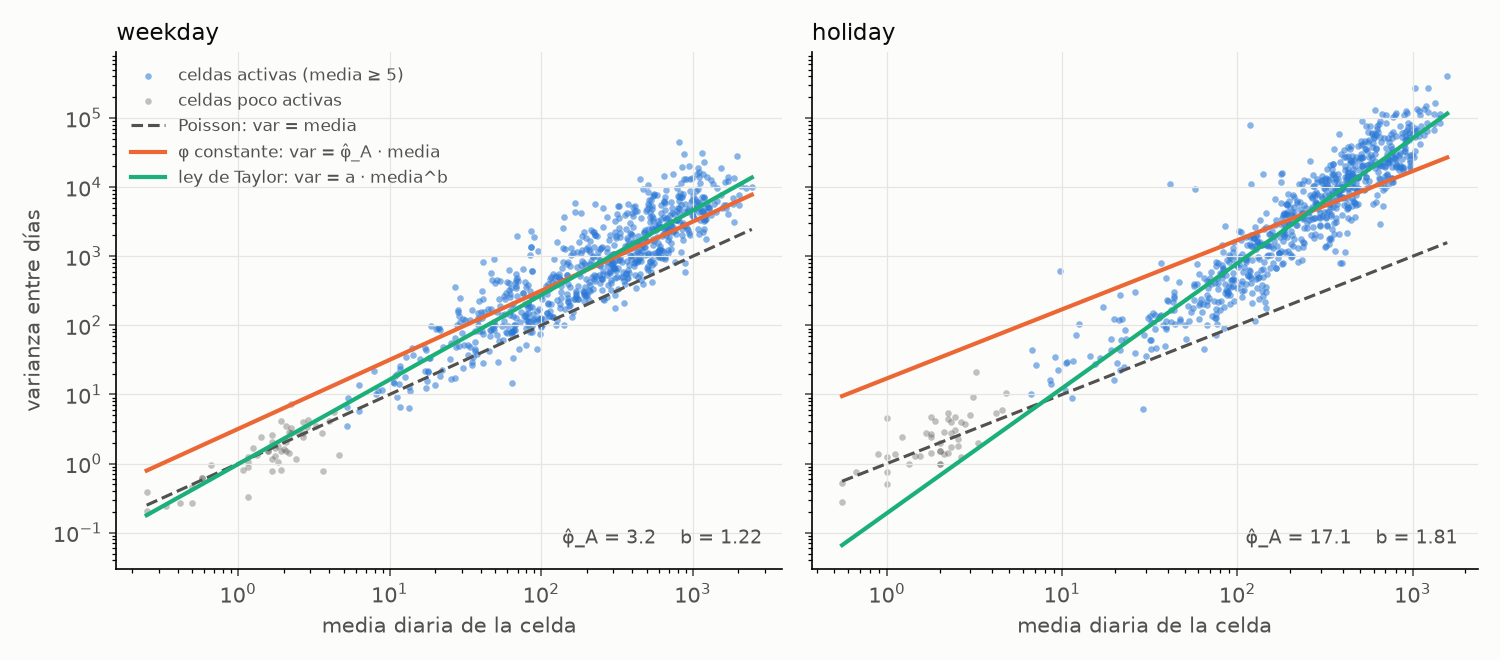
\includegraphics[width=\textwidth]{figs/Chap3/sobredispersion_media_varianza.png}
\caption{Varianza entre días frente a media diaria de cada celda, en escala
logarítmica. La recta discontinua es la de Poisson; la naranja, un modelo
cuasi-Poisson con $\varphi$ constante; la verde, la ley de potencia
$\mathrm{var} = a\,\mu^b$ ajustada a las celdas activas.}
\label{fig:prop-dispersion}
\end{figure}

\begin{enumerate}
  \item \textbf{La sobredispersión es sustancial.} La varianza de una celda
  típica es 3 veces su media en el periodo laborable y 17 veces en el feriado.
  Con la nula de Poisson, la prueba rechazaría la independencia por esta sola
  razón.
  \item \textbf{No es constante y crece con el volumen.} En escala logarítmica,
  la varianza crece con pendiente $b > 1$, y el cociente var/media pasa de 2.8 en
  las celdas poco activas a 49 en las más activas del periodo feriado. Un modelo
  cuasi-Poisson con un único $\hat\varphi$ corregiría de más los bloques poco
  activos y de menos los de mucho volumen, que son los que concentran la masa. Con
$\hat\varphi = 17.1$, la mediana del feriado, una celda poco activa con cociente
2.8 se corregiría de más unas seis veces, y una muy activa con cociente 49.1 se
corregiría de menos casi tres veces.
  \item \textbf{Una parte no afecta a la prueba, y otra es correlacionada.} Si
  la intensidad de un día se multiplica por un factor común a toda la ciudad, a
  una región o a un intervalo, por ejemplo $\mu_{dij} = a_i\, b_j\,
  \gamma_{di}$, la suma sobre los días
  $\sum_d \mu_{dij} = a_i \bigl(\sum_d \gamma_{di}\bigr) b_j$ sigue siendo un
  producto de un efecto de fila y uno de columna, y la independencia dentro del
  bloque se conserva. Por ejemplo, con $a=(1,2)$ y $b=(10,20)$, si en el día 1 el
factor es $\gamma_{1i}=(1,1)$ y en el día 2 es $\gamma_{2i}=(2,0.5)$, de modo que
la primera región está muy activa y la segunda poco, la suma sobre los dos días da
$(30,60)$ para la primera región y $(30,60)$ para la segunda, filas proporcionales
y, por tanto, ningún patrón falso. El caso $\gamma_{dj}$ es simétrico. Al eliminar esos
  efectos con el modelo log-lineal sin interacción triple, con términos
  día--región, día--intervalo y región--intervalo, la dispersión residual baja a
  2.1 y 6.7, y sigue creciendo con el volumen. Lo que queda proviene de la
  variación propia de cada celda y de la combinación de efectos
  día--región y día--intervalo, que produce desviaciones correlacionadas entre
  las celdas de un bloque, con la forma de una interacción, cuyo peso en
  $G^2_B$ crece con la masa del bloque.
\end{enumerate}

El tercer hecho tiene una consecuencia de diseño, a saber, que una nula que trate cada celda
por separado, aunque use una función de varianza que crezca con la media
(Sección~\ref{sec:est-efecto}), no puede reproducir esas desviaciones
correlacionadas. La nula de AST-CC se construye, por eso, con los días
completos, de modo que cada réplica conserva la correlación que existe entre las
celdas de un mismo día, y esa es la propiedad que justifica el procedimiento que
se describe a continuación.

\subsection{Distribución nula mediante \emph{bootstrap} de días}\label{sec:prop-bootstrap}

Todas las pruebas se calibran por simulación, de modo que se generan $B_{\mathrm{perm}}$
tablas nulas del bloque, se calcula en cada una el estadístico $t_b$ y, con el
estadístico observado $t_{\mathrm{obs}}$, el p-valor es
\begin{equation}\label{eq:prop-pval}
  p = \frac{1 + \#\{b : t_b \ge t_{\mathrm{obs}}\}}{1 + B_{\mathrm{perm}}},
\end{equation}
que incluye la tabla observada entre las réplicas y nunca vale cero
\cite{Phipson2010}. Con $B_{\mathrm{perm}}=199$ y cuatro réplicas por encima del
valor observado, el p-valor es $5/200 = 0.025$, y si ninguna lo supera es
$1/200 = 0.005$, que es el mínimo que esa cantidad de réplicas permite alcanzar.

Las réplicas se generan con los propios días observados, aplicando el principio
del \emph{bootstrap} bajo la hipótesis nula (Sección~\ref{sec:est-bootstrap}), de modo
que se remuestrean los días, pero alrededor de la media de independencia del bloque y
no de los datos observados. Para cada celda del
bloque con media diaria $\bar X_{ij}\ge 0.5$ se define la fluctuación
multiplicativa del día $d$, $F_{dij} = X_{dij}/\bar X_{ij}$, y su versión
corregida por muestra pequeña
\begin{equation}\label{eq:prop-fluctuacion}
  \tilde F_{dij} = \max\Bigl\{0,\ 1 + \sqrt{\tfrac{D}{D-1}}\,\bigl(F_{dij}-1\bigr)\Bigr\},
\end{equation}
que compensa que la varianza empírica de $D$ días subestima la poblacional. Si
el recorte en cero actúa, las $\tilde F_{dij}$ de la celda se reescalan para que
su media vuelva a ser uno. En las celdas con menos actividad el cociente no es
fiable: se toma $\tilde F_{dij}=1$ y la réplica de la celda se sortea como
Poisson con la media que le corresponde, de modo que conserve al menos esa
variabilidad. Para una celda con
cuatro días de conteos $(80,100,90,130)$ y media 100, las fluctuaciones son
$(0.8,1.0,0.9,1.3)$ y, con el factor $\sqrt{4/3}\approx1.155$, las corregidas son
$(0.77,1.00,0.88,1.35)$, que multiplican por $4/3$ la varianza de las
fluctuaciones. Cada réplica sortea
$D$ días $d_1,\dots,d_D$ con reemplazo y toma
\begin{equation}\label{eq:prop-bootstrap}
  O^{(b)}_{ij} = \frac{E^B_{ij}}{D}\sum_{k=1}^{D} \tilde F_{d_k ij},
\end{equation}
redondeado a un entero de forma estocástica, sin sesgo. En la celda anterior, si
$E^B_{ij}=400$ y se sortean los días $(4,1,4,2)$, la suma de las fluctuaciones
corregidas es $4.46$ y la réplica vale $400/4\cdot4.46\approx446$. La media de las réplicas
es la de independencia en el bloque, $E^B$, así que cumplen el nulo. Si un día
solo difiere de los demás por un factor común a todo el bloque, a una región o
a un intervalo, la fluctuación es de rango uno y la réplica sigue siendo
independiente, como exige el tercer hecho de la sección anterior; la combinación
de efectos y la variación propia de cada celda, en cambio, se trasladan tal como
aparecen en los datos. El método no supone ninguna forma para la varianza ni
para la correlación entre celdas, pero sí que los días son independientes y que
$E^B$ estima bien las medias. Además del p-valor, las réplicas proporcionan la
media $\bar t_0$ del estadístico bajo el nulo, que se usa para corregir el sesgo
del tamaño de efecto (Sección~\ref{sec:prop-parada}) sin costo adicional.

\paragraph{Evidencia preliminar de calibración.} Para elegir esta nula se
compararon varias alternativas sobre datos nulos semirreales, que consisten, para cada bloque
base de ST-CC, en 300 réplicas generadas con \eqref{eq:prop-bootstrap} a partir de
los días reales, las cuales cumplen la independencia por construcción pero tienen la
variabilidad de los datos. Cada prueba se aplicó solo con los $D$ días de cada
réplica y con 199 réplicas propias. La Tabla~\ref{tab:prop-calibracion} resume
el error de tipo~I resultante al nivel 0.05.

\begin{table}[t]
\centering
\small
\begin{tabular}{@{}lcccc@{}}
\toprule
 & \multicolumn{2}{c}{Laborable (24 bloques)} & \multicolumn{2}{c}{Feriado (24 bloques)} \\
\cmidrule(lr){2-3}\cmidrule(l){4-5}
Nula & Media & Máximo & Media & Máximo \\
\midrule
Poisson (Patefield) & 0.40 & 0.84 & 0.76 & 1.00 \\
Cuasi-Poisson, $\hat\varphi$ constante & 0.03 & 0.19 & 0.01 & 0.06 \\
Gamma--Poisson con $\mathrm{var} = a\,\mu^b$ & 0.02 & 0.11 & 0.06 & 0.42 \\
\emph{Bootstrap} de días, sin corrección & 0.06 & 0.14 & 0.11 & 0.39 \\
\emph{Bootstrap} de días \eqref{eq:prop-bootstrap} & 0.04 & 0.13 & 0.09 & 0.33 \\
\bottomrule
\end{tabular}
\caption{Error de tipo~I de la prueba ómnibus al nivel 0.05 sobre datos nulos
semirreales construidos con los días de noviembre de 2017. Para cada bloque base
de ST-CC se usaron 300 réplicas; el error de Monte Carlo por bloque es de
aproximadamente 0.013.}
\label{tab:prop-calibracion}
\end{table}

La nula de Poisson rechaza la independencia verdadera en el 40\,\% de los casos
en el periodo laborable y en el 76\,\% en el feriado. Las nulas que tratan las
celdas por separado son conservadoras en la mayoría de los bloques, lo que cuesta
potencia, y liberales en los de más volumen. El \emph{bootstrap} de días con la
corrección \eqref{eq:prop-fluctuacion} es el único cuyo error se centra en el
nominal en el periodo laborable, con media 0.044 y mediana 0.042.

En el periodo feriado, el generador de la tabla mezcla al azar sábados, domingos
y el Día de Acción de Gracias, mientras que la matriz real tiene siempre la
misma composición. Con un generador que la respeta, el error medio del \emph{bootstrap}
baja a 0.045, aunque 5 de los 24 bloques, casi todos nocturnos y de dos
intervalos, siguen por encima del nominal, con un máximo de 0.30. Remuestrear los
días dentro de cada tipo de día no lo mejora, ya que con solo cuatro sábados y cuatro
domingos, el error medio sube a 0.11. AST-CC usa, por tanto, el \emph{bootstrap} sin
estratos en ambos periodos, y la liberalidad residual en los bloques nocturnos
del periodo feriado se trata como una limitación conocida
(Sección~\ref{sec:prop-limitaciones}). Como estos datos nulos semirreales
comparten su mecanismo con el \emph{bootstrap}, lo que puede favorecerlo, la
calibración del método completo se medirá también con datos sintéticos de
mecanismo distinto (Capítulo~\ref{chap:resultados}).

\subsection{Corrección por la búsqueda del mejor corte}\label{sec:prop-minP}

El corte que se prueba fue elegido porque maximiza la separación. Si su
estadístico se comparara con la distribución $\chi^2$ de un corte fijado de
antemano, el p-valor estaría fuertemente sesgado hacia cero. Con siete candidatos
independientes de un grado de libertad, por ejemplo, la probabilidad de que al
menos uno supere el umbral del 5\,\% es $1-0.95^7\approx 0.30$, y no 0.05; los
candidatos reales están correlacionados, por lo que el sesgo es menor, pero con
las 2047 biparticiones de columnas sigue siendo grande. Este es el
problema de doble uso de los datos que \cite{Gao2024} documentan para el
agrupamiento jerárquico.

AST-CC lo corrige con un ajuste de tipo \emph{min-P} \cite{Westfall1993}, que
consiste en que en cada réplica nula se repite la búsqueda completa del mejor corte y se
registra su estadístico máximo. El p-valor \eqref{eq:prop-pval} compara así el
máximo observado con la distribución del máximo bajo el nulo, lo que ajusta a
la vez por el número de candidatos y por la correlación entre ellos, con más
potencia que una corrección de Bonferroni sobre todos los candidatos. Omitir la
repetición de la búsqueda invalida el p-valor, como lo muestra una comprobación
preliminar con bloques nulos de los tamaños de los bloques base, en la que comparar
el mejor corte de
filas con la $\chi^2$ de un corte fijo produjo errores de tipo~I de hasta 0.98
al nivel 0.05, mientras que con el ajuste \emph{min-P} el error medio fue 0.053.
Las pruebas dirigidas reutilizan las réplicas que ya generó la prueba ómnibus, y
sobre cada una se repiten las tres búsquedas. Cada prueba sigue siendo válida
por separado, y el costo de generar réplicas se paga una sola vez por bloque.

\subsection{Alcance de la corrección}

La repetición de la búsqueda corrige la selección del corte dentro de un nodo,
pero no la selección del propio nodo. Los bloques base provienen de BBAC$_I$ y
los bloques hijos provienen de cortes elegidos con los mismos datos. Esto importa porque BBAC$_I$ elige la partición base de modo que sus grupos sean
lo más distintos posible entre sí, de manera que los bloques resultantes tienden a
parecer heterogéneos aunque los datos no tengan estructura, y algo análogo ocurre
con cada corte aceptado, que se eligió por separar bien los datos que luego se
usan para probarlo. Por eso,
la validez de las pruebas en los nodos no puede darse por supuesta aunque cada
prueba individual esté bien calibrada, y el
Capítulo~\ref{chap:resultados} incluye un experimento de calibración sobre datos
nulos que mide cuántos refinamientos espurios produce el método completo al
nivel nominal, con la partición base estimada a partir de los mismos datos.

\section{Control de comparaciones múltiples}\label{sec:prop-multiplicidad}

Un árbol de refinamiento implica muchas pruebas, a saber, una por cada bloque base
y, en cascada, una por cada hijo. Aplicar el mismo nivel $\alpha$ a todas ellas
produciría muchos falsos refinamientos, y dividir $\alpha$ entre el número total
de pruebas, como hace SigTree con la corrección de Bonferroni \cite{Hu2025},
ignora la estructura jerárquica y resulta demasiado conservador. Con veinte
pruebas independientes al 5\,\%, la probabilidad de al menos un falso rechazo es
$1-0.95^{20}\approx 64$\,\%, y Bonferroni la evita dando a todas el mismo nivel
$0.05/20 = 0.0025$ aunque unos bloques tengan muchos más datos que otros.

AST-CC reparte el nivel global $\alpha$ de arriba abajo, en proporción a la masa
de cada bloque, siguiendo la lógica de las pruebas jerárquicas de
\cite{Meinshausen2008} y de \cite{Kimes2017},
\begin{equation}\label{eq:prop-alpha}
  \alpha_{B_{gh}} = \alpha\,\frac{N_{B_{gh}}}{N}\quad\text{(bloques base)},
  \qquad
  \alpha_{C} = \alpha_B\,\frac{N_C}{N_B}\quad\text{(hijos } C\in\mathcal{C}(B,s_B)\text{)},
\end{equation}
y un bloque solo se prueba si su padre fue refinado. El reparto por masa da
prioridad automática a los bloques con más datos, y los niveles de los bloques
que nunca se visitan no se gastan. Con $N=10\,000$ viajes, $\alpha=0.05$ y cuatro
bloques base de 4000, 3000, 2000 y 1000 viajes, los niveles son 0.020, 0.015, 0.010
y 0.005, que suman 0.05. Si el bloque de 4000 se corta en hijos de 3000 y 1000
viajes, estos reciben 0.015 y 0.005, que suman lo que tenía el padre. El bloque
grande trabaja entonces con 0.02, ocho veces el nivel de 0.0025 de Bonferroni, lo
que es razonable porque tiene más datos y más potencia.

El argumento de control es el siguiente. Si el nulo de independencia se cumple
en un bloque, se cumple en todos sus sub-bloques, así que los nulos verdaderos
forman subárboles completos. Un falso rechazo ocurre por primera vez en la raíz
de alguno de esos subárboles, y esas raíces son bloques disjuntos cuyos niveles
suman como máximo $\alpha$. En el ejemplo anterior, si los bloques de 2000 y 1000
viajes fueran verdaderamente nulos, la probabilidad de refinarlos por error sería a
lo sumo $0.010+0.005=0.015\le 0.05$. Si cada prueba fuera válida a su nivel y la
jerarquía estuviera fijada de antemano, la tasa de error por familia (FWER), que es
la probabilidad de al menos un falso refinamiento en todo el árbol, sería, por lo
tanto, a lo sumo $\alpha$. Como la jerarquía se construye con los
datos, la garantía es aproximada, y su comportamiento real es parte del
experimento de calibración mencionado en la sección anterior.

El reparto \eqref{eq:prop-alpha} tiene una consecuencia práctica, ya que el nivel de un
bloque pequeño puede ser inferior a la resolución $1/(B_{\mathrm{perm}}+1)$ de
un p-valor por simulación. Por eso el número de réplicas se adapta a cada
bloque, $B_{\mathrm{perm}}(B) = \max\{B_{\min},\ \lceil c/\alpha_B\rceil\}$,
acotado por un máximo $B_{\max}$ que limita el costo. Con los valores de
referencia, un bloque con $\alpha_B=0.02$ usa 199 réplicas, uno con $\alpha_B=0.005$
usa 400 y uno con $\alpha_B=0.0001$ llega al máximo de 20\,000. Si incluso con $B_{\max}$
réplicas el p-valor mínimo $1/(B_{\max}+1)$ supera $\alpha_B$, el bloque no
puede rechazarse y se marca como hoja inalcanzable, para distinguirla de
una hoja homogénea. Además se aplica la parada secuencial de \cite{Besag1991},
en la que la simulación se detiene en cuanto se acumulan $h$ réplicas con estadístico
mayor o igual que el observado. Las réplicas se generan por lotes de 500 y la regla se
evalúa al cierre de cada lote, de modo que el p-valor es la proporción de réplicas que
igualan o superan al observado en las generadas hasta ese momento. Con
$B_{\mathrm{perm}}\le 500$ la regla no se activa y se usan todas las réplicas, lo que
es barato porque la prueba ómnibus solo requiere calcular $G^2$ sobre cada tabla;
el ahorro está en los bloques con $\alpha_B$ muy pequeño, que exigen miles de
réplicas, donde un bloque claramente no significativo se abandona tras el primer
lote. Si el bloque supera la prueba ómnibus, la simulación se completó
y sus réplicas sirven para las pruebas dirigidas.

\section{Criterios de parada}\label{sec:prop-parada}

Con matrices de millones de viajes, casi cualquier desviación de la
independencia resulta significativa. Los propios \cite{Hu2025} señalan que el
estadístico $\chi^2$ crece con el tamaño de la muestra y dificulta el control de
los falsos descubrimientos. Por eso AST-CC exige la significancia y un
tamaño de efecto mínimo, nunca solo una de las dos. Un bloque con un millón de
viajes e información mutua de 0.0005 nats por observación tiene $G^2 = 1000$, un
p-valor prácticamente nulo, y una interacción irrelevante; otro con mil viajes e
información mutua de 0.05 tiene $G^2=100$, y si pasa la prueba también supera el
umbral de efecto. La significancia crece con el número de viajes y el tamaño de
efecto no. La Tabla~\ref{tab:prop-parada} reúne todos los criterios.

\begin{table}[t]
\centering
\small
\begin{tabular}{>{\raggedright\arraybackslash}p{0.2\textwidth}>{\raggedright\arraybackslash}p{0.3\textwidth}>{\raggedright\arraybackslash}p{0.4\textwidth}}
\toprule
Criterio & Condición para ser hoja & Justificación \\
\midrule
Tamaño mínimo & $|I|<2$ o $|J|<2$ & Con una sola fila o columna, $G^2_B=0$, de modo que no hay interacción posible. \\
Masa mínima & $N_B<N_{\min}$ & Evita probar bloques con muy poca actividad. \\
Profundidad máxima & $d\ge d_{\max}$ & Acota el costo y la complejidad del árbol. \\
Nivel inalcanzable & $1/(B_{\max}+1)>\alpha_B$ & Con el máximo de réplicas, la prueba no podría rechazar. \\
Significancia & $p_{\mathrm{omn}}>\alpha_B$, o ningún corte con p-valor $\le\alpha_B$ & No hay evidencia de heterogeneidad, o no puede localizarse. \\
Tamaño de efecto & $\tilde I_B<\delta$ & La interacción residual es irrelevante aunque sea detectable. \\
Ganancia del corte & $\tilde g_{B,s}<\delta$ & El corte explica demasiado poca información. \\
\bottomrule
\end{tabular}
\caption{Criterios de parada de AST-CC. Los cuatro primeros son reglas que no
dependen de la estructura interna del bloque, análogas a las de SigTree \cite{Hu2025}; los
tres últimos son estadísticos.}
\label{tab:prop-parada}
\end{table}

El umbral $\delta$ es la defensa principal contra la inflación por tamaño de
muestra. Tiene una interpretación directa, información mutua en nats por
observación, y no crece con $N$. En los datos de esta tesis es, además, el que
decide el refinamiento en los primeros niveles del árbol, ya que con masas de unos mil
a cientos de miles de viajes por bloque, el cociente $G^2_B/\nu_B$ de los
bloques base de ST-CC va de 3 a más de 1700, y la prueba de independencia
rechaza en prácticamente todos ellos. La prueba cobra importancia en los bloques
pequeños y profundos, donde la masa es menor.

\paragraph{Tamaño de efecto corregido por sesgo.} La información mutua empírica
está sesgada hacia arriba en los bloques pequeños
(Sección~\ref{sec:est-efecto}). Aunque no haya interacción,
$\mathrm{E}[G^2_B]\approx\nu_B = (|I|-1)(|J|-1)$ bajo Poisson, y más con
sobredispersión, de modo que $\mathrm{E}[\hat I_B]\approx \nu_B/(2N_B) > 0$. En el
periodo laborable, por ejemplo, un bloque de 1033 viajes y 12 grados de
libertad tiene $\hat I_B = 0.017$, el quinto valor más alto de los 24 bloques,
y cerca de un tercio de esa cantidad ($12/2066\approx 0.006$) es la que se
esperaría solo por el ruido de Poisson. Si además la media de $G^2$ bajo el nulo
fuera, por la sobredispersión, de unas 25 unidades en lugar de 12, el mismo
bloque tendría un tamaño de efecto corregido de $(35.1-25)/2066\approx 0.005$, lo
que muestra cuánto depende la lectura del ruido que se descuente; el valor de 25 es
ilustrativo. AST-CC usa, por eso, las versiones
corregidas
\begin{equation}\label{eq:prop-efecto-corregido}
  \tilde I_B = \max\Bigl\{0,\ \frac{G^2_B - \bar t_0}{2N_B}\Bigr\},
  \qquad
  \tilde g_{B,s} = \max\Bigl\{0,\ \frac{G^2_{B,s} - \bar t_{0,s}}{2N_B}\Bigr\},
\end{equation}
donde $\bar t_0$ es la media de $G^2_B$ sobre las réplicas nulas de la prueba
ómnibus y $\bar t_{0,s}$ la media del estadístico dirigido
\eqref{eq:prop-dirigidos} sobre las mismas réplicas. Ambas medias se obtienen de
réplicas que ya se generan para los p-valores, así que la corrección no tiene
costo. Como las réplicas siguen el \emph{bootstrap} de días, $\bar t_0$ incorpora la
variabilidad real entre días; y como $\bar t_{0,s}$ se calcula repitiendo la
búsqueda, descuenta también el optimismo de elegir el mejor corte.

\paragraph{Elección de $\delta$.} Su valor no se fija a priori. Como referencia
de escala, la información mutua $\hat I_B$ de los bloques base de ST-CC va de
0.0012 a 0.061 nats en el periodo laborable y de 0.0017 a 0.19 en el feriado.
En el Capítulo~\ref{chap:resultados} se recorre una rejilla que cubre ese rango,
por ejemplo $\delta\in\{0.001, 0.0025, 0.005, 0.01, 0.02\}$, y para cada valor
se reportan el número de hojas, la fracción del término de interacción local de
ST-CC que explica el árbol según el Corolario~\ref{cor:stcc},
$\sum_{B\in\mathcal{S}}G^2_{B,s_B}\big/\sum_{g,h}G^2_{gh}$, y la estabilidad de
las hojas. Como medida estandarizada complementaria puede reportarse la $V$ de
Cramér de cada hoja.

\section{Algoritmo}\label{sec:prop-algoritmo}

Los Algoritmos~\ref{alg:astcc} y \ref{alg:mejorcorte} reúnen los elementos
anteriores. La Tabla~\ref{tab:prop-parametros} resume los parámetros del método,
junto con los valores de referencia que se usarán en los experimentos y que se
someterán a un análisis de sensibilidad, como se indica en su última columna. El
Algoritmo~\ref{alg:astcc} describe el procedimiento recursivo completo, desde la
partición base hasta la decisión sobre cada bloque, y el
Algoritmo~\ref{alg:mejorcorte} detalla cómo se selecciona el mejor corte y se
calcula su p-valor con el ajuste \emph{min-P}.

\begin{algorithm}[t]
\caption{Refinamiento jerárquico de ST-CC con AST-CC}\label{alg:astcc}
\begin{algorithmic}[1]
\Require Matriz de conteos $O\in\mathbb{N}^{m\times n}$ y sus días $X_1,\dots,X_D$; $K_R$, $K_T$; nivel $\alpha$; umbral $\delta$; $N_{\min}$, $d_{\max}$; y los demás parámetros de la Tabla~\ref{tab:prop-parametros}
\Ensure Árbol de refinamiento $\mathcal{T}$
\State $(\rho,\tau)\gets$ BBAC$_I(O, K_R, K_T)$ con base C5 y búsqueda local \Comment{partición base}
\ForAll{bloque base $B_{gh}$}
  \State \Call{Refinar}{$B_{gh},\ \alpha N_{B_{gh}}/N,\ 0$}
\EndFor
\State \Return $\mathcal{T}$
\Statex
\Procedure{Refinar}{$B=I\times J,\ \alpha_B,\ d$}
  \If{$|I|<2$ \textbf{o} $|J|<2$ \textbf{o} $N_B<N_{\min}$ \textbf{o} $d\ge d_{\max}$}
    \State marcar $B$ como hoja; \Return
  \EndIf
  \State $B_{\mathrm{perm}}\gets\min\{B_{\max},\ \max\{B_{\min},\ \lceil c/\alpha_B\rceil\}\}$
  \If{$1/(B_{\mathrm{perm}}+1)>\alpha_B$}
    \State marcar $B$ como hoja inalcanzable; \Return
  \EndIf
  \State calcular $G^2_B$ con \eqref{eq:prop-G2}
  \State generar réplicas $O^{(b)}$ con \eqref{eq:prop-bootstrap}, por lotes, hasta $B_{\mathrm{perm}}$ o hasta que al cierre de un lote $h$ superen $G^2_B$ \Comment{la parada solo se activa si el bloque no es significativo}
  \State $(p_{\mathrm{omn}}, \bar t_0)\gets$ p-valor y media nula de $G^2_B$ sobre las réplicas
  \State $\tilde I_B\gets\max\{0,\ (G^2_B-\bar t_0)/(2N_B)\}$
  \If{$p_{\mathrm{omn}}>\alpha_B$ \textbf{o} $\tilde I_B<\delta$}
    \State marcar $B$ como hoja homogénea; \Return
  \EndIf
  \State $(s_{\mathrm{fil}},p_{\mathrm{fil}},\bar t_{\mathrm{fil}})\gets$ \Call{MejorCorte}{$B,\ \text{filas},\ \{O^{(b)}\}$}
  \State $(s_{\mathrm{col}},p_{\mathrm{col}},\bar t_{\mathrm{col}})\gets$ \Call{MejorCorte}{$B,\ \text{columnas},\ \{O^{(b)}\}$}
  \If{$\min(p_{\mathrm{fil}},p_{\mathrm{col}})\le\alpha_B$}
    \State $s\gets$ corte de menor p-valor (desempate por $z$)
  \Else
    \State $(s_{\mathrm{conj}},p_{\mathrm{conj}},\bar t_{\mathrm{conj}})\gets$ \Call{MejorCorte}{$B,\ \text{conjunto},\ \{O^{(b)}\}$}
    \If{$p_{\mathrm{conj}}>\alpha_B$}
      \State marcar $B$ como hoja heterogénea no localizada; \Return
    \EndIf
    \State $s\gets s_{\mathrm{conj}}$
  \EndIf
  \State $\tilde g_{B,s}\gets\max\{0,\ (G^2_{B,s}-\bar t_{0,s})/(2N_B)\}$ \Comment{$\bar t_{0,s}$ es la media nula del tipo de $s$}
  \If{$\tilde g_{B,s}<\delta$}
    \State marcar $B$ como hoja heterogénea no localizada; \Return
  \EndIf
  \ForAll{$C\in\mathcal{C}(B,s)$}
    \State \Call{Refinar}{$C,\ \alpha_B N_C/N_B,\ d+1$}
  \EndFor
\EndProcedure
\end{algorithmic}
\end{algorithm}

\begin{algorithm}[t]
\caption{Selección del mejor corte con ajuste \emph{min-P}}\label{alg:mejorcorte}
\begin{algorithmic}[1]
\Function{MejorCorte}{$B,\ \text{tipo},\ \{O^{(b)}\}_{b=1}^{B_{\mathrm{perm}}}$}
  \State $s^\ast\gets$ \Call{Buscar}{$O|_B,\ \text{tipo}$} \Comment{Sección~\ref{sec:prop-candidatos}}
  \State $t_{\mathrm{obs}}\gets G^2_{B,s^\ast}$
  \For{$b=1,\dots,B_{\mathrm{perm}}$}
    \State $s_b\gets$ \Call{Buscar}{$O^{(b)},\ \text{tipo}$} \Comment{se repite la búsqueda completa}
    \State $t_b\gets G^2_{B,s_b}$ calculado sobre $O^{(b)}$
  \EndFor
  \State $p\gets \bigl(1+\#\{b: t_b\ge t_{\mathrm{obs}}\}\bigr)/\bigl(1+B_{\mathrm{perm}}\bigr)$
  \State $\bar t\gets$ media de los $t_b$ \Comment{para \eqref{eq:prop-efecto-corregido}}
  \State \Return $(s^\ast, p, \bar t)$
\EndFunction
\end{algorithmic}
\end{algorithm}

\begin{table}[t]
\centering
\small
\begin{tabular}{>{\raggedright\arraybackslash}p{0.18\textwidth}>{\raggedright\arraybackslash}p{0.4\textwidth}>{\raggedright\arraybackslash}p{0.32\textwidth}}
\toprule
Parámetro & Papel & Valor de referencia \\
\midrule
$K_R$, $K_T$ & Resolución inicial de la partición base & Los de \cite{Liu2021}; sensibilidad en el Cap.~\ref{chap:resultados} \\
Inicializaciones de BBAC$_I$ & Ejecuciones de la partición base, cada una con búsqueda local & $200$, como \cite{Liu2021} \\
$\alpha$ & Nivel global (FWER sobre el árbol) & $0.05$ \\
$\delta$ & Información mutua mínima por observación, corregida por sesgo & Rejilla en $[0.001, 0.02]$ nats; sensibilidad \\
$N_{\min}$, $d_{\max}$ & Reglas triviales de parada & $500$ viajes y profundidad $6$; sensibilidad \\
$B_{\min}$, $c$, $B_{\max}$ & Réplicas mínimas, resolución respecto de $\alpha_B$ y máximo & $199$, $2$ y $20\,000$ \\
$h$ & Parada secuencial de Besag y Clifford, evaluada por lotes de 500 réplicas & $10$ \\
Límites de enumeración & Tamaño máximo para buscar cortes por enumeración & $|I|\le14$; $|J|\le6$ en el corte conjunto \\
$R_{\mathrm{ini}}$ & Inicializaciones del 2-medias para bloques con más de 14 filas & $10$ \\
$\kappa$ & Índice de Jaccard mínimo para la frecuencia de soporte & $0.5$ como punto de partida \\
\bottomrule
\end{tabular}
\caption{Parámetros de AST-CC.}
\label{tab:prop-parametros}
\end{table}

Los parámetros de la tabla son de dos tipos. Los que condicionan el resultado y
por eso se someten a análisis de sensibilidad son $K_R$, $K_T$, $\alpha$, $\delta$,
$N_{\min}$ y $d_{\max}$, que son decisiones del investigador. Los demás
(inicializaciones, número de réplicas, parada secuencial y límites de enumeración)
son técnicos y buscan dar fiabilidad a las pruebas sin ser el foco de la
interpretación. Un recorrido del Algoritmo~\ref{alg:astcc} con números ayuda a
verlo. Sea $N=10\,000$, $\alpha=0.05$ y un bloque base de 4000 viajes, con nivel
$\alpha_B=0.02$. El bloque supera las reglas triviales y su número de réplicas es
$\min\{20\,000,\max\{199,\lceil 2/0.02\rceil\}\}=199$, con un p-valor mínimo de
$1/200=0.005\le 0.02$, de modo que la prueba es alcanzable. Si la prueba ómnibus da
$p_{\mathrm{omn}}=0.005$ y $\tilde I_B=0.03\ge\delta=0.005$, el bloque pasa la
puerta. Si además $p_{\mathrm{fil}}=0.005$ y $p_{\mathrm{col}}=0.4$, solo el corte de
filas es significativo y se acepta cuando su ganancia corregida supera $\delta$. Si
deja hijos de 3000 y 1000 viajes, estos reciben niveles de 0.015 y 0.005, y el segundo
usa $\max\{199,400\}=400$ réplicas antes de repetir el mismo procedimiento. El
criterio de nivel inalcanzable de la Tabla~\ref{tab:prop-parada} usa $B_{\max}$ y el
algoritmo usa $B_{\mathrm{perm}}$, que está acotado por $B_{\max}$; ambos coinciden,
porque si $\alpha_B$ es grande la prueba es alcanzable y si es pequeño
$B_{\mathrm{perm}}$ llega a $B_{\max}$.

\subsection{Costo computacional}

La partición base cuesta lo mismo que ST-CC, $O(mn(K_R+K_T))$ por iteración de
BBAC$_I$ y por inicialización, más la búsqueda local; esta última puede evaluar
cada movimiento de una fila o columna en $O(K_R K_T)$, porque con las bases C2 y
C5 la divergencia depende solo de los totales de bloque. El costo adicional se
concentra en las pruebas por simulación. En un bloque $B=I\times J$, cada
réplica requiere generar una tabla de $|I|\times|J|$ y repetir las búsquedas. La
de columnas evalúa $2^{|J|-1}-1$ tablas colapsadas de $|I|\times2$, y la de
filas, mientras $|I|\le 14$, $2^{|I|-1}-1$ tablas de $2\times|J|$. El costo por
bloque es del orden de
\[
  O\Bigl(B_{\mathrm{perm}}(B)\,\bigl[\,2^{|J|}|I| + 2^{\min(|I|,14)}|J|\,\bigr]\Bigr),
\]
más el del corte conjunto, que solo se evalúa cuando ningún corte
unidimensional es significativo. Con $n=12$ y bloques base de a lo sumo quince
filas, los dos términos exponenciales están acotados por constantes moderadas. Un
bloque de 10 filas y 12 columnas requiere del orden de $2^{12}\cdot10+2^{10}\cdot12
\approx 5\cdot10^4$ operaciones elementales por réplica, y uno de 14 filas, unas
$2.5\cdot10^5$, de modo que con 199 réplicas el trabajo es del orden de $10^7$ y
$5\cdot10^7$ operaciones respectivamente. Estas cifras son órdenes de magnitud y
no tiempos medidos, que se reportarán junto con los resultados del
Capítulo~\ref{chap:resultados}.
Tres propiedades mantienen el costo total manejable. La primera es que la parada
secuencial abandona pronto los bloques no significativos; la segunda, que los
bloques de un mismo nivel son independientes dado el árbol, por lo que se
procesan en paralelo; y la tercera, que el tamaño de los bloques decrece con la
profundidad.

\section{Representación e interpretación de los resultados}\label{sec:prop-representacion}

La partición de ST-CC se lee como $K_T$ patrones espaciales con su dinámica
temporal y $K_R$ patrones temporales con su distribución espacial. Con
refinamiento local, esa lectura deja de existir como objeto único, porque la
partición temporal puede cambiar de un subconjunto de regiones a otro. Para no
perder interpretabilidad, AST-CC acompaña el árbol de cinco productos.

\paragraph{Descriptores de hoja.} Para cada hoja $L = I_L\times J_L$ se reportan
sus regiones y horarios, su masa $N_L$, su interacción residual $\tilde I_L$ (solo
para las hojas que llegaron a la prueba ómnibus, pues requiere las réplicas nulas), su
tipo (homogénea, heterogénea no localizada, inalcanzable o trivial, esta última por
las reglas de tamaño, masa o profundidad de la Tabla~\ref{tab:prop-parada}) y su nivel de
actividad relativo
\begin{equation}\label{eq:prop-lift}
  \ell_L = \frac{N_L}{\sum_{(i,j)\in L} O_{i\cdot}\,O_{\cdot j}/N},
\end{equation}
que compara la actividad observada en la hoja con la que predicen los volúmenes
globales de sus regiones e intervalos. Un valor $\ell_L>1$ indica que ese grupo
de regiones se activa en ese grupo de horarios más de lo que corresponde a su
volumen, y un valor $\ell_L<1$, que está más apagado de lo que corresponde. Por
ejemplo, con $N=10\,000$ y una hoja formada por dos regiones de 500 y 300 viajes
totales y dos horarios de 1000 y 2000, el esperado es
$800\cdot3000/10\,000=240$, y si la hoja tiene 360 viajes, $\ell_L=1.5$. La referencia es el modelo de independencia de toda la matriz y no el
del bloque padre, ya que este último reproduce los totales de fila y de columna del
padre, de modo que, tras un corte de filas o de columnas, el cociente respecto
del padre vale exactamente uno en todos los hijos y no distingue nada. Un bloque
de 4000 viajes cortado en hijos de 3000 y 1000 daría $3000/3000=1$ y
$1000/1000=1$ respecto de su padre.

\paragraph{Árbol anotado.} Cada nodo interno muestra el tipo de corte, la
ganancia corregida $\tilde g_{B,s}$ y el p-valor, de modo que se lee qué parte de la
heterogeneidad fue espacial y qué parte temporal. Esta representación conserva la
trazabilidad de las decisiones, ya que cada hoja puede leerse como el resultado de
la secuencia de cortes que llevó hasta ella, de manera análoga a la lectura de las
reglas de un árbol de decisión. Si un bloque base se corta por filas y uno de
sus hijos se corta después por columnas, la hoja resultante se lee como un grupo
de regiones, dentro de ese bloque, en un grupo de horarios, donde la primera
pregunta fue espacial y la segunda temporal.

\paragraph{Matriz teselada.} La matriz se reordena según la partición base y,
dentro de cada bloque, según sus cortes, y se dibuja con los contornos de las
hojas y un color proporcional a $\ell_L$, como en la
Figura~\ref{fig:prop-teselacion}. De este modo se obtiene una vista global en la
que los patrones locales aparecen como rectángulos de color distinto dentro de
bloques que, en el tablero de ST-CC, se mostraban uniformes.

\paragraph{Mapas de profundidad.} Para cada región se representa en el mapa la
profundidad máxima que alcanza el refinamiento en sus filas, y análogamente para
cada intervalo de tiempo. Si una región aparece en hojas de profundidades 1, 3 y 2,
su valor en el mapa es 3. Estos mapas indican dónde y cuándo la partición base
resulta insuficiente. Un mapa con profundidad uniforme indicaría que el tablero de
ST-CC era suficiente, mientras que las zonas con profundidades altas señalan las
regiones y los horarios donde se concentra la interacción espacio-temporal local.

\paragraph{Frecuencia de soporte.} Como BBAC$_I$ converge a mínimos locales y
el refinamiento es voraz, cada hoja se acompaña de su frecuencia de soporte,
que es la proporción de ejecuciones, con distintas inicializaciones de la partición
base, en que aparece una hoja con índice de Jaccard, medido sobre celdas,
mayor o igual que $\kappa$ respecto de ella. El índice de Jaccard entre dos
conjuntos de celdas es el cociente entre el tamaño de su intersección y el de su
unión, y vale 1 si son idénticos y 0 si no comparten ninguna. Una hoja de $3\times2$
celdas y otra de $2\times2$ contenida en ella tienen un índice de $4/6\approx0.67$,
de modo que no se cuentan como la misma hoja con $\kappa=0.7$ y sí con
$\kappa=0.5$. Una hoja con soporte bajo, por ejemplo la que aparece en menos de la
mitad de las ejecuciones, no debe interpretarse como hallazgo.

\section{Alcance y limitaciones del diseño}\label{sec:prop-limitaciones}

Varias limitaciones se derivan directamente de las decisiones de diseño y
conviene explicitarlas antes de los experimentos, porque condicionan tanto la
interpretación de los resultados como el diseño de las comparaciones que se
presentarán en el Capítulo~\ref{chap:resultados}. Cada una se describe a
continuación junto con la forma en que se piensa evaluar su efecto.

\begin{itemize}
  \item \textbf{Restricción guillotina.} El refinamiento solo mira hacia
  dentro de cada bloque. Un patrón local que cruce la frontera entre dos
  bloques base no puede recuperarse como una sola hoja, sino como hojas
  separadas en cada bloque. Por ejemplo, un patrón en las regiones 3 a 6 en las
  mismas horas, con las regiones 3 y 4 en un bloque base y las 5 y 6 en otro, se
  recupera como dos hojas pequeñas y no como un rectángulo de cuatro regiones.
  \item \textbf{Dependencia de la partición base.} El refinamiento parte de un
  óptimo local de BBAC$_I$, cuyo paisaje tiene muchos mínimos locales; la
  búsqueda local y las múltiples inicializaciones lo atenúan, y la frecuencia
  de soporte (Sección~\ref{sec:prop-representacion}) mide su efecto sobre las
  hojas. La elección de la base también importa, ya que con C5 y con C2 se obtienen
  tableros muy distintos, y C5 deja menos interacción local por refinar, porque
  agrupa las regiones por la forma de su perfil y no por su volumen.
  \item \textbf{Resolución de entrada.} Los cortes agrupan regiones e
  intervalos, pero no los subdividen, de modo que el método no puede bajar de la resolución
  espacial y temporal de la matriz. Los resultados dependen, por tanto, de la
  zonificación usada, que en el caso de las zonas de taxi de Nueva York tiene
  tamaños muy dispares.
  \item \textbf{Parámetros.} El método no elimina $K_R$ y $K_T$, sino que
  cambia su papel, pues fijan la resolución inicial, mientras que la resolución
  final la deciden $\alpha$ y $\delta$, dos parámetros con interpretación
  directa. Esta afirmación solo se sostiene si el resultado final es
  razonablemente estable frente a $K_R$ y $K_T$, lo que debe comprobarse
  empíricamente.
  \item \textbf{Comparación con rejillas más finas.} Cabe preguntar por qué
  no basta con aumentar $K_R$ y $K_T$ o elegirlos con Cross-Associations
  \cite{Chakrabarti2004}. La respuesta debe ser empírica, y consiste en comprobar que una rejilla global con
  el mismo número de parámetros, o con el mismo valor de \eqref{eq:prop-bic},
  no recupera los patrones locales que encuentra AST-CC. La diferencia en el
  número de parámetros ilustra el argumento. Con $n=12$ intervalos repartidos en
  $K_T=4$ grupos de tres columnas, un corte de filas en un único bloque añade
  $|J|-1=2$ parámetros, mientras que partir globalmente el mismo grupo de filas a
  lo largo de los cuatro grupos de columnas añade $4\cdot2=8$.
  \item \textbf{Validez de las pruebas.} La selección de los nodos a partir de
  los datos puede inflar el error de tipo~I. El \emph{bootstrap} de días supone que
  los días son independientes y usa $E^B$ como estimación de las medias; con
  pocos días, como en el periodo feriado, es algo liberal en los bloques
  nocturnos. Por eso es indispensable un experimento de calibración sobre datos
  nulos.
  \item \textbf{Costo frente a resolución.} El reparto del nivel por masa hace
  que los bloques con muy pocos viajes reciban niveles menores que la
  resolución alcanzable con $B_{\max}$ réplicas. Esos bloques quedan como hojas
  inalcanzables, ya que el método no afirma que sean homogéneos, sino que no puede
  probarlos al nivel asignado. Con $N=10^6$ y $\alpha=0.05$, por ejemplo, un
  bloque de 600 viajes recibe $\alpha_B=3\cdot10^{-5}$; supera el mínimo de masa,
  pero el p-valor más pequeño que alcanza con 20\,000 réplicas es
  $1/20\,001\approx5\cdot10^{-5}$, mayor que su nivel.
  \item \textbf{Significativo no es interesante.} Una hoja puede tener
  heterogeneidad detectable y ser irrelevante en el dominio. Por eso se reporta
  siempre el tamaño de efecto junto al p-valor, y los patrones principales se
  contrastan con conocimiento del dominio, como el foco alrededor de Penn
  Station que identifican \cite{Liu2021}.
\end{itemize}

\paragraph{Extensiones que quedan como trabajo futuro.} Varias alternativas se
consideraron durante el diseño y quedan fuera del alcance de esta tesis.
Entre ellas se encuentra el control jerárquico de la tasa de falsos descubrimientos de
\cite{Yekutieli2008}, más permisivo que la FWER cuando se esperan muchos
refinamientos, que se dejó fuera porque la FWER es la garantía más simple de
interpretar en una primera versión del método. Otra es una variante que elija la
partición y los cortes con la mitad de los días y los pruebe con la otra mitad, lo
que elimina el doble uso de los datos a costa de potencia, en la línea del
\emph{count splitting} de \cite{Neufeld2024cs}, y que exige antes comprobar que la
mitad de los días basta para estimar la partición. También se consideraron nulas
paramétricas con una función de varianza por celda, como la ley de potencia de
\cite{Taylor1961}, que no se adoptaron porque, como muestra la
Sección~\ref{sec:prop-calibracion}, no reproducen las desviaciones correlacionadas
entre las celdas de un bloque. Los cortes de columnas podrían restringirse a
intervalos consecutivos, lo que reduciría las 2047 biparticiones posibles con doce
intervalos a solo 11 y daría patrones más fáciles de interpretar, a costa de no
capturar horarios no contiguos, como las dos horas punta del día. Por último, un
paso posterior de fusión de hojas vecinas recuperaría los patrones que cruzan
bloques base, que es la limitación de la restricción guillotina.

\section{Consideraciones Finales}\label{sec:prop-final}

Este capítulo presentó AST-CC, una extensión de ST-CC que refina localmente la
partición en tablero mediante un árbol de cortes guiados por pruebas de
hipótesis. La pieza teórica central es la
Proposición~\ref{prop:ganancia}, según la cual, bajo el modelo de independencia por hoja, la
divergencia del árbol se descompone exactamente entre las hojas y la ganancia de
cada corte es un estadístico de razón de verosimilitud. Con ella, el
Corolario~\ref{cor:stcc} muestra que el método descompone, de forma controlada,
el término de interacción local que ST-CC deja sin modelar, de modo que el
criterio de refinamiento y la función objetivo de ST-CC son la misma cantidad
vista a distintas escalas.

Sobre esa base, el método combina una prueba ómnibus calibrada con un \emph{bootstrap}
de los días observados, que reproduce su variabilidad real; pruebas dirigidas
que localizan la estructura con un ajuste \emph{min-P} que repite la búsqueda en cada
réplica; un reparto jerárquico del nivel de significancia a lo largo del árbol;
y un umbral de tamaño de efecto, corregido por sesgo, que no crece con el número
de viajes y que, a la escala de estos datos, es el que decide el refinamiento.
Las limitaciones identificadas, en particular la validez aproximada de las
pruebas cuando la jerarquía se construye con los datos, orientan directamente
el diseño experimental del Capítulo~\ref{chap:resultados}, donde el método se
evalúa sobre datos sintéticos con patrones locales conocidos, sobre datos nulos
y sobre los datos de taxis de Manhattan. Cada limitación tiene allí una forma de
evaluarse, que es la calibración sobre datos nulos para la validez de las pruebas,
la comparación con rejillas globales de igual número de parámetros para el valor del
refinamiento local, y el análisis de sensibilidad a $K_R$, $K_T$, $\alpha$ y
$\delta$ para la dependencia de la partición base y de los parámetros.
